%%%%%%%%%%%%%%%%%%%%%%%%%%%%%%%%%%%%%%%%%
% Masters/Doctoral Thesis 
% Version 1.43 (17/5/14)
%
% This template has been downloaded from:
% http://www.LaTeXTemplates.com
%
% Original authors:
% Steven Gunn 
% http://users.ecs.soton.ac.uk/srg/softwaretools/document/templates/
% and
% Sunil Patel
% http://www.sunilpatel.co.uk/thesis-template/
%
% License:
% CC BY-NC-SA 3.0 (http://creativecommons.org/licenses/by-nc-sa/3.0/)
%
% Note:
% Make sure to edit document variables in the Thesis.cls file
%
%%%%%%%%%%%%%%%%%%%%%%%%%%%%%%%%%%%%%%%%%

%----------------------------------------------------------------------------------------
%	PACKAGES AND OTHER DOCUMENT CONFIGURATIONS
%----------------------------------------------------------------------------------------

\documentclass[11pt, oneside]{Thesis} % The default font size and one-sided printing (no margin offsets)

\graphicspath{{Images/}} % Specifies the directory where pictures are stored

\usepackage{listings}
\usepackage{color}
\usepackage{comment}
\usepackage[norsk]{babel}
\usepackage{wrapfig}
\usepackage{lipsum}



\addto\captionsnorsk{% Replace "english" with the language you use
  \renewcommand{\contentsname}%
    {Innhold}%
}

\definecolor{dkgreen}{rgb}{0,0.6,0}
\definecolor{gray}{rgb}{0.5,0.5,0.5}
\definecolor{mauve}{rgb}{0.58,0,0.82}


\lstset{frame=tb,
  language=C++,
  aboveskip=3mm,
  belowskip=3mm,
  showstringspaces=false,
  columns=flexible,
  basicstyle={\small\ttfamily},
  numbers=none,
  numberstyle=\tiny\color{gray},
  keywordstyle=\color{blue},
  commentstyle=\color{dkgreen},
  stringstyle=\color{mauve},
  breaklines=true,
  breakatwhitespace=true,
  tabsize=3
}

\usepackage{pdfpages}
\usepackage[square, numbers, comma, sort&compress]{natbib}
\usepackage{mathtools}
\usepackage[table,xcdraw]{xcolor}
\usepackage{epigraph}
\usepackage{enumitem}
\usepackage{nameref}
\usepackage{listings}
\usepackage{changepage}


\newenvironment{steps}[1]{\begin{enumerate}[label=#1 \arabic*]}{\end{enumerate}}

\makeatletter% http://tex.stackexchange.com/questions/29517/forcing-new-line-after-item-number-in-enumerate-environment/29518#29518
\def\step{%
   \@ifnextchar[ \@step{\@noitemargtrue\@step[\@itemlabel]}}
\def\@step[#1]{\item[#1]\mbox{}\\\hspace*{\dimexpr-\labelwidth-\labelsep}}
\makeatother


\renewcommand{\epigraphflush}{center}

\usepackage{dirtree}

\newcommand\tab[1][1cm]{\hspace*{#1}}

%\usepackage{apacite}
%\usepackage[natbibapa]{apacite}
\hypersetup{urlcolor=black, colorlinks=true} % Colors hyperlinks in blue - change to black if annoying.

\title{\ttitle} % Defines the thesis title - don't touch this

\begin{document}


\frontmatter % Use roman page numbering style (i, ii, iii, iv...) for the pre-content pages

\setstretch{1.3} % Line spacing of 1.3

% Define the page headers using the FancyHdr package and set up for one-sided printing
\fancyhead{} % Clears all page headers and footers
\rhead{\thepage} % Sets the right side header to show the page number
\lhead{} % Clears the left side page header

\pagestyle{fancy} % Finally, use the "fancy" page style to implement the FancyHdr headers

\newcommand{\HRule}{\rule{\linewidth}{0.5mm}} % New command to make the lines in the title page

% PDF meta-data
\hypersetup{pdftitle={\ttitle}}
\hypersetup{pdfsubject=\subjectname}
\hypersetup{pdfauthor=\authornames}
\hypersetup{pdfkeywords=\keywordnames}


\makeatletter
\renewcommand{\@chapapp}{Kapittel}
\makeatother

\renewcommand{\contentsname}{Innhold}
%\renewcommand{\listoffigures}{Figurer}
%\renewcommand{\bibname}{Referanser}

%----------------------------------------------------------------------------------------
%	TITLE PAGE
%----------------------------------------------------------------------------------------

\begin{titlepage}
\begin{center}

%\textsc{\LARGE \univname}\\[1.5cm] % University name
\includegraphics[scale=1.5]{logo} \\[1.5cm]
\HRule \\[0.4cm] % Horizontal line
{\huge \bfseries \ttitle}\\[0.4cm] % Thesis title
\HRule \\[1.5cm] % Horizontal line
 
\begin{minipage}{0.4\textwidth}
\begin{flushleft} \large
\emph{Student:}\\
{\authornames} % Author name - remove the \href bracket to remove the link
\end{flushleft}
\end{minipage}
\begin{minipage}{0.4\textwidth}
\begin{flushright} \large
\emph{Veileder:} \\
{\supname}\\ % Supervisor name - remove the \href bracket to remove the link  

\end{flushright}
\end{minipage}\\[3cm]
 

\textit{Ved}\\[0.4cm]
\groupname\\\univname\\[4cm] % Research group name and department name
 
{\large \today}\\[4cm] % Date
%\includegraphics{logo} % University/department logo - uncomment to place it
 
\vfill
\end{center}


\end{titlepage}

%\includepdf[pages=-,landscape=false,offset=75 -75, pagecommand={\thispagestyle{fancy}}]{./Appendices/obligegen.pdf}


\begin{adjustwidth*}{2cm}{2cm}
\let\clearpage\relax
\chapter{Sammendrag}
Dette prosjektet har gått ut på å utvikle en nettside for bedriften Rusta Vrak Bilutleige. Denne nettsiden skal fungere som et bestillingsverktøy for kunder som ønsker å leie bil, og for at bedriften skal ha et verktøy for å holde styr på alle utleier til enhver tid. I dag har Rusta Vrak Bilutleige en enkel informasjonsnettside uten noen form for funksjonalitet, og har derfor et ønske om å kunne tilby sine kunder et alternativt digitalt bestillingsverktøy.
 
I tillegg til selve utviklingen skulle prosjektet også publiseres på nett. Til dette formålet har det blitt benyttet en metode for publisering i en skytjeneste. Her ble leverandøren Google  benyttet, og på deres platform som kalles Google App Engine. Ved å benytte en slik publiseringsmetode ble det mer tid til arbeid med selve nettsiden.


\end{adjustwidth*}




\newpage
%----------------------------------------------------------------------------------------
%	LIST OF CONTENTS/FIGURES/TABLES PAGES
%----------------------------------------------------------------------------------------

\pagestyle{fancy} % The page style headers have been "empty" all this time, now use the "fancy" headers as defined before to bring them back

\lhead{\emph{Innhold}} % Set the left side page header to "Contents"
\tableofcontents % Write out the Table of Contents

%\lhead{\emph{List of Figures}} % Set the left side page header to "List of Figures"
\listoffigures % Write out the List of Figures


%\lhead{\emph{List of Tables}} % Set the left side page header to "List of Tables"
%\listoftables % Write out the List of Tables

%----------------------------------------------------------------------------------------
%	THESIS CONTENT - CHAPTERS
%----------------------------------------------------------------------------------------

\mainmatter % Begin numeric (1,2,3...) page numbering

\pagestyle{fancy} % Return the page headers back to the "fancy" style

% Include the chapters of the thesis as separate files from the Chapters folder
% Uncomment the lines as you write the chapters


\lhead{Introduksjon}
\chapter{Innlending}
\section{Bakgrunn}
%Rusta Vrak bilutleige er et lite firma basert i Førde og Jøster i Sogn og Fjordane. Utleie firmaet blir driftet av verkstedmesteren Stein Olav Erikstad, og målet er å kunne tilby utleie av greie og fult funksjonelle biler til en rimelig pris. Firmaet ble startet i 2013, og har i dag en flåte på over 20 biler. Rusta Vrak fungerer i dag som et sideprosjekt, men det har gode muligheter for vekst i fremtiden, men dersom et bilutleige firma ønsker å være kompetitivt, er det viktig å kunne tilby en digital form for tilgjengelighet på lik linje som de mer etablerte bedriftene. Derfor har Rusta Vrak Bilutleige uttryket ønske om å få en 


%I tillegg til selve utviklingen, skulle også prosjektet publiseres og gjøres tilgjengelig på internett. Til dette formålet har det blitt benyttet en metode for publisering i skytjenesten til Google, på plattformen Google App Engine. Ved å benytte en slik publiseringsmetode kunne det settes av mer tid til selve utviklingen av selve nettsiden.

Rusta Vrak Bilutleige er et lite firma basert i Førde og Jølster i Sogn og Fjordane. Målet til bedriften er å kunne tilby utleie av greie og fult funksjonelle biler til en rimelig pris. Bedriften ble startet i 2013, og blir driftet av verkstedmesteren Stein Olav Erikstad. Rusta Vrak Biltuleige fungerer som et sideprosjekt, men har gode muligheter for vekst i fremtiden, og dersom et lite bilutleie firma skal være kompetitivt på markedet, er det viktig å kunne tilby digitale bestillingsmuligheter på lik linje som de større og mer etablerte. Derfor har Rusta Vrak Bilutleige uttrykt et ønske om å få en ny nettside knyttet til bedriften.


\section{Problemdefinisjon}
Rusta Vrak Bilutleie har i dag en nettside basert på tjenesten Blogspot [CITATION], dette er en enkel informasjonsside som oppgir informasjon om bilene, priser og kontaktinformasjon. Deretter må kunden ta kontakt enten vha. telefon eller epost for å foreta selve bestilling. Da firmaet blir driftet av én person som et sideprosjekt, kan det være vanskelig å alltid være tilgjengelig, og samtidig ha en oversikt over hvilke biler som er ledige til enhver tid. Dette kan bli forbedret ved å gjøre nettsiden til firmaet mer interaktiv både for kunde og bedrift. 

\subsection{Oppgaven}
%Lag en nettside for bilutleie firmaet Rusta Vrak Bilutleige. Denne nettsiden skal kunne benyttes av kunder for å finne hvilke biler som passer best for kundens formål, få en oversikt over når de spesifikke bilene er ledige for utleie, og foreta en reservasjon av valgt bil.

Lag en nettside for bilutleie firmaet Rusta Vrak Bilutleige. Denne nettsiden skal kunne benyttes av kunder som et bestillingsverktøy. Dette inkl. mulighet til å se hvilke biler som er tilgjengelig for leie, når de individuelle biler er ledig, og foreta en reservasjon gjennom internett.

%Nettsiden skal også kunne benyttes av firmaet for å få en oversikt over bilene som er klar for utleie, kunder som leier eller har leid bil. Det må være mulig å legge til, fjerne og redigere bilene for utleie forløpende.

Nettsiden skal også kunne benyttes av firmaet for å få en oversikt over bilene som er klar for utleie, samt gi en oversikt over kunder som leier og de som har leid bil tidligere. Det må være mulig å legge til, fjerne og redigere bilene som ligger for utleie forløpende.


\subsection{Krav} \label{kravliste1}
I samarbeid med firmaet ble det utarbeidet en liste over krav som var viktig å få med i produktet. Denne kravlisten ble brukt som grunnmuren av planleggingsfasen av prosjektet. 
%I samarbeid med firmaet utarbeidet vi noen krav over hva som er viktig å få med i nettsiden.
\begin{description}
\item[Lett å bruke.]Nettsiden skal være enkel å bruke, og skal helst være så intuitiv som mulig. Det betyr at den ikke skal for komplisert i bruk.
\item[Skalering mellom skjermstørrelser.]Gjøre nettsiden like god å bruke på smartphone som på PCer.
\item[Selvstendig og Billig.]Firmaet er lite, og derfor skal nettsiden kunne være så selvstendig som mulig. Dvs. arbeid med drift og opprettholdning skal være minimal. Utover dette burde hosting av nettsiden også være rimelig.
\item[Håndere alle reservasjoner.]Nettsiden skal både fungere som et bestillingsverktøy for kunder, og som et oversiktsverktøy for bedriften. Derfor skal brukere kunne benytte nettsiden for reservasjoner, og ansatte skal ha et administrasjons område hvor det er mulig å legge til nye reservasjoner manuelt.
\item[Fordel å leie i lange perioder.]Det skal være en fordel å leie over lengre perioder. Systemet må ta hensyn til dette og det skal implementeres en funksjon for å kalkulere prisen i forhold til dette.
\end{description}

\section{Litteratur Studie}
Det aller meste av studie mot denne oppgaven har foregått på internett. Dette inkluderer hovedsakelig bruk av dokumentasjonen til de forskjellige rammeverker og plattformer. Utover dette har det blitt benyttet noen bøker som har fungert som oppslagsverk gjennom hele prosessen.

\subsubsection*{Bøker}
\begin{itemize}
\item Code Complete 2. Edition (Steve McConnel)
\item Programming Google App Engine with Python (Dan Sanderson)
\item HTML and CSS Design and Build Websites (Jon Duckett)
\end{itemize}


\section{Problemløsning}
\subsection{Prosjekt Plan} \label{kravliste2}
Det første som ble gjort mot denne oppgaven var å lage en plan over alle funksjoner og arbeidsoppgaver som må med i det endelige produktet, og legge disse inn i kategorier basert på viktighet. Kategoriene går fra 1 til 5, og planen var å gå stegvis gjennom denne listen. 
 \begin{enumerate}
 
  \item \textbf{Oppsett og Installasjon}
  \begin{enumerate}
  	\item \textbf{Lokalt Utviklingsmiljø} - Installere Python, oppsett av virtualenv, Installere og integrere JetBrains PyCharm, installere rammeverket Django.
  	\item \textbf{Lokal Database} - Installasjon og opprette kobling mellom Django prosjekt og lokal MySQL database.
  	\item \textbf{Google Cloud Platform} - Installering og oppsett av kobling mellom lokalt prosjekt og Google Cloud Platform. Dette inkluderer både hosting og database
  \end{enumerate}
  
  \item \textbf{Første Steg i Utviklingen}
  \begin{enumerate}
  	\item \textbf{Database Tabeller} - Planlegging og oppretting av database modeller og tabellene.
  	\item \textbf{Forside} - Enkel forside.
  	\item \textbf{Admin} - Mulighet til å legge til / slette biler fra opprettet database.
  	\item \textbf{Generere Liste over Biler fra Database} - Basert på biltype.
  	\item \textbf{Bil Reservasjon} - Mulighet å legge inn er reservasjon av bil som går mellom to datoer.
  \end{enumerate}
  
  \item \textbf{Videreutvikling}
  \begin{enumerate} 
  	\item \textbf{Bilder} - Mulighet for å kunne vise bilde av bilene. Både som thumbnail og alternativt galleri.
	\item \textbf{Kalender} - Gjør det mulig for kunde å ha visuell oversikt når den spesifikke bilen er ledig for utleie. 
	\item \textbf{Epost Bekreftelse} - Send en email til kunde som reserverer. Denne skal inneholde nyttig informasjon om reservasjonen.
	\item \textbf{Reservasjon Håndtering} - Legg til funksjonalitet som stopper en reservasjon fra å krasje med annen allerede eksisterende reservasjon.
	\item \textbf{Søkefunskjon} - Finne ledige biler på dato.
  \end{enumerate}
  
  \item \textbf{Ekstra Funksjonalitet}
	\begin{enumerate}
		\item \textbf{Pris Funksjon} - Det skal være en fordel å leie over lengre perioder. Derfor må en funksjon kunne dele ut riktig mengde rabatt over hvor mange dager som er i leieperioden. Videre skal denne kunne runde til nærmeste 5 for å slippe unødvendig småpenger.
		\item \textbf{PDF} - Mulighet å laste ned PDF med bestillingsdetaljer.
		\item \textbf{Filtrering av Bil Listen} - F.eks. kun biler som har automat. 
		\item \textbf{Konfigurering av Admin} - Søk bil på skiltnr. Oversikt over alle reservasjoner og kunde informasjon.
	\end{enumerate}
  \item \textbf{Dersom tid}
  	\begin{enumerate}
  	\item \textbf{Google Calendar} - Legg til informasjon i en Google Calendar for enkel oversikt over når biler hentes og leveres.
  	\end{enumerate}
 
 \end{enumerate}
 
 
\subsection{Arbeidsmetode} \label{chap:method}
Utviklingen av dette prosjektet har benyttet en iterativ og inkrementell arbeidsmetode. Denne metoden går ut på å gjennomføre utviklingen stegvis, man begynner utviklingen med et skjelett, som man vil videre legge til litt funksjonalitet, og deretter komme tilbake og legge til mer på toppen av dette igjen. Ved å benytte en slik prosess, blir det mulig å utvikle flere områder på nettsiden samtidig uten at det nødvendigvis krasjer med hverandre i prosessen.

En iterativ metode gjør det mulig å splitte et større prosjekt i mindre, mer håndterlige biter. Planlegging, design, utvikling av kode og testing blir gjennomført i gjenntatte sykluser \cite{method:iterative_fig}. Dermed kan man følge figur \ref{fig:iterative_development} for prosessen gjennom hele utviklingen.

 \begin{figure}[htbp]
	\centering
		\includegraphics[scale=0.5]{Bilder/iterativ_utvikling.png}
	\caption[Iterativ Utviklings Diagram]{Oversikt over trinnene per syklus i iterativ utvikling \cite{iterative:development}. } %\ref{fig:iterative}
	\label{fig:iterative_development}
\end{figure}



\subsection{Rapportens Struktur}
Denne rapporten har blitt delt inn i 5 kapitler.

Første kapittel introduserer bakgrunn og problemet som skal løses. Her finner man en kravliste utarbeidet i samarbeid med bedriften, og en planlagt fremgangsmåte for å kunne møte disse kravene. Deretter finner man kapittelet som beskriver de valgte teknologiene, og presenterer en liten oversikt over disse. Etter dette kommer kapittelet om selve løsningen, og her vil det endelige resultatet av prosjektet komme frem. Man får her et overblikk over hvordan nettsiden fungerer, både fra et brukerperspektiv, og et administrerende perspektiv. Så finner man et kapittel som diskuterer oppgaven, her drøftes det litt om hvorvidt målet har blitt møtt, og litt om fremtidig arbeid. Til slutt finner man konklusjonen for prosjektet.

Alle relevante vedlegg som vises til i rapporten finner man på de siste sidene.





\newpage
\chapter{Oversikt over valgte Teknologier}

\section{Publisering}
Ett av kravene til prosjektet var at nettsiden skal være så selvstendig som mulig. Det skal være minimalt med nedetid, serveren må kunne oppdateres uten manuelt inngrep og backup av database må foregå automatisk. Samtidig som å oppfylle dette burde selve hostingen være så billig som mulig. Derfor ble det noe moderne konseptet av Platform as a Service benyttet.

\subsection{Platform as a Service}
En Platform as a Service (PaaS) er et utviklings og distribusjons miljø basert i en skytjeneste \cite{ paas:azure}. En PaaS leverandør har som ansvar å levere og opprettholde en utviklings og distribusjons plattform for sine kunder. De har videre ansvaret på områdene rundt konfigurering, oppsett av servere og sikkerhet på server siden. Det er populært å referere til  PaaS leverandører som IT-avdelingen til produktet, som gjør at utvikleren kan fokusere mer på selve utviklingen enn oppsett av infrastrukturen som ligger under \cite[s. 10]{bachelor}

\subsection{Fordeler ved PaaS}
\subsubsection*{Spare Tid}
Utviklingen foregår direkte mot arkitekturen til den valgte skytjenesten, derfor vil man unngå forarbeidet rundt oppsett og installasjon av servere. Dersom en server hos PaaS leverandøren skulle gå offline, vil dette bli ordnet fortløpende av leverandøren, uten at man som kunde må gripe inn \cite[s. 9]{bachelor}.

\subsubsection*{Billig}
Samtidig som å levere mye i pakken, kan publisering vha. PaaS være billig. Dette kommer av at de aller fleste leverandørene bruker dynamisk ressursallokering. Det betyr at ressursene allokert til et prosjekt vil følge samme kurve som behovet. Ved lite eller ingen trafikk vil et prosjekt gå i dvalemodus og bli der helt til en forespørsel blir sendt til serveren. Man betaler kun for de ressurser som blir benyttet.

\subsection{Valg av PaaS Leverandør}
PaaS er fortsatt et moderne konsept, og man har mange muligheter ved valg av leverandør. Det er en enorm jobb å foreta en sammenlikning over de relevante mulighetene, derfor har jeg valgt å gå ut ifra et studie som jeg foretok under et bachelor prosjekt våren 2016 \cite[s. 18]{bachelor}. Her ble det utført en sammenlikning av 3 av de største PaaS leverandørene: Google Cloud Platform, Microsoft Azure og Amazon Web Services. 


\subsection*{Resultat}
Alle de tre nevnte leverandørene har et bredt utvalgt av muligheter på sine løsninger. Alle tilbyr et løfte av server tilgjengelighet på 99,95\% av tiden. De har gode tilkoblingsmuligheter i Europa og prisen er basert på tid og ressurser.

Men det er spesielt ett område de har unike løfter; Gratis Kvoter. \\
Microsoft Azure leverer kun gratis kvoter i form av trial account. Her får man ressurser for 200\$ som man kan benytte som man selv bestemmer, i løpet av de første 30 dager etter Trial Account blir opprettet.\\
Amazon  Web Services kommer utstyrt med 1 år ‘free tier’, som inneholder 5GB lagringsplass, 20 000 GET requests og 2 000 Put Requests.\\
Google Cloud Platform derimot tilbyr daglige gratis kvoter. Dette inkluderer bl.a. 28 Frontend Instance timer\footnote{Google Cloud Platforms ‘frontend instance’ blir opprettet ved at en applikasjon får en forespørsel, og denne instance vil være tilgjengelig for bruk de neste 15 minutter. Alle nye forespørsler i disse neste 15 minutter vil benytte samme frontend instance}, 1GB plass for lagring av logger, 1GB data inn og ut.


Ved å bruke Google Cloud Platforms gratis kvoter, vil man kunne ha hosting av mindre trafikkerte nettsider bortimot gratis, og man behøver kun betale for databasen.\\
\textbf{Valg: Google Cloud Platform}



\newpage
\section{Programmeringsspråk og Rammeverk}
Med dette prosjektet ville jeg videreutvikle min kompetanse innen bruken av web-applikasjons rammeverket Django, basert på programmeringsspråket Python. 
\subsection{Python}
Python er et skriptingspråk utviklet av nederlandske Guide van Rossum. Den tidligste versjonen kom frem i 1996 og det har stadig vært i utvikling siden. Python har et formål om å gjøre kode leselig og gjenbrukbar, og har et mindre fokus på ren hastighet. Utover dette har Python et fokus på å gjøre utviklingen, og debuggings fasene av prosjekter så raskt som mulig \cite[s. 11]{bachelor}.
\subsection{Django}

\begin{wrapfigure}{r}{4.5cm}
\caption[Django Oversikt]{Stegene Django kjører gjennom ved et HTML request. }\label{wrap-fig:1}
\includegraphics[width=4.5cm]{Bilder/django.png}
\end{wrapfigure}

Django er et web-applikasjons rammeverk som kommer levert med en ‘batterier inkuldert' filosofi. Dette betyr at vanlig funksjonalitet som ofte blir benyttet i en web sammenheng blir levert med i grunnpakken til Django. Dette inkluderer bruker-system, URL routing, template system, administrasjons system og database object-relational mapper (ORM) \cite{django:what}.





På figur \ref{wrap-fig:1} kan man se en oversikt over hvordan Django håndterer et HTML request. 

Først vil den tyde hvilke URL som kommer inn. Django inneholder et register over tilgjengelige URL som kan benyttes vha. regular expressions. Den vil sjekke dette registeret og finne hvilken funksjon (view) som tilhører den innkommende URL.

Den korresponderende funksjon i view vil nå håndtere data fra HTML requestet, dette innebærer å sjekke om det er et POST eller GET request, og hente ut eventuell data med henyn til dette. 

Data vil bli hentet vha. Djangos Modeller, som er et objekt orientert metode å fremstille den tilkoblede databasen. Når det er klart hvilke data som skal hentes, vil Djangos ORM konvertere Djangos Database API til SQL Query. Den data som resulterer fra spørringen vil bli returnert tilbake til view.

Til slutt vil view samle data og generere den tilhørende template (html), som videre sendes tilbake til browseren.



\section{Front-end}
På front-end aspektet av nettsiden har det i hovedsak blitt benyttet 2 biblioteker som bør nevnes.  

\subsection{Bootstrap}
Bootstrap ble først laget av en designer og utvikler hos Twitter i 2010, og har fått stort følge siden. Det er i dag ett av de største og mest populære front-end rammeverkene i verden. Da det er så mye brukt, vil det da være et større følge aktive brukere på nettsider som stackoverflow.com, som videre gjør det mer attraktivt å bruke.

\subsubsection{Skalerbart}
Boostrap kommer utstyrt med et Grid system. Dette systemet er basert på å dele opp skjermen inn seksjoner, basert på skjermstørrelsen. Dette gir muligheten av å kunne spesifisere hvordan et element skal oppføre seg i forhold til skjermstørrelsen, dette resulterer i en nettside som fungerer like godt på smartphones, tablets og PCer.

\subsubsection{Komponenter}
Rammeverket kommer med en hel rekke komponenter som kan benyttes.  Dette gjelder bl.a. en rekke valg innen navigasjonsmenyer, input bokser, knapper etc. Disse komponentene er videre fult mulig å redigere vha. CSS.


\subsection{JQuery}


\section{Verktøy}
\begin{description}
\item[GitHub]ble benyttet som versjons kontroll underveis i utviklingen. For hver nye feature som skulle introduseres, ble dette utviklet på en egen branch. Når utviklingen av en ny feature fungerte som planlagt, skulle den testes grundig før den ble pushet over på Master branch.
\item[Google App Engine SDK.] Google Cloud Platform kommer utstyrt med en SDK når man skal arbeide mot Google App Engine. Denne SDK inneholder et lokalt utviklingsmiljø som kjører på samme infrastruktur som det benyttet ved hostingen. Man får også publisering og administrasjons muligheter direkte vha. enkel GUI. Denne har hovedsakelig blitt brukt som et test område underveis i utviklingen, samt. Publisering av nyere versjoner etter hvert som nettsiden har blitt oppdatert.
\item[JetBrains PyCharm] har blitt brukt som IDE. Denne inneholder en bred rekke hjelpemidler for å gjøre utviklingsprosessen smidigere. Den støtter både utvikling av Django prosjekter og html/css/javascript. I tillegg har den et godt system for autocomplete av kode, og vil generere hint for forbedringer av bl.a. navn på funksjoner, indentering og sørger for at all kode benytter samme navn konvensjon.
\item[LateX.]Under rapportskrivingen har typesettingssystemet LateX blitt brukt får å generere dokumentet. Dette systemet hjelper med å skape en god utforming av hele dokumentet, som gir bedre muligheter for å fokusere på selve skrivingen. LateX gir et såkalt WYSIWYM (What You See Is What You Mean), som beskriver en form for skriving hvor det resulterende dokument bedre representerer den faktiske informasjonen man arbeider med.



\end{description}


\chapter{Løsning}
\lhead{Løsning}

\section{Krav}
For å se kravlistene \ref{kravliste1} og \ref{kravliste2} 



Utifra denne kravlisten ble et workflow en bruker skal benytte ved bestilling av bil laget:
WORKFLOW!!

\subsection{Workflow}
En kunde skal kunne benytte nettsiden som et bestillingsverktøy. %Kunden skal selv ha kontroll på hvordan han finner frem til bilen som passer best. %Hovedsakelig skal man ha 2 alternativer: 
%Søke basert på dato i leieperioden og biltype, \textbf{eller} se en komplett liste over alle biler, evt. basert på kategori. 
\subsubsection{Fremgangsmåte}
\begin{steps}{Steg}
\step \textbf{Forside}\\Man starter med å se på forsiden av nettsiden. Denne skal inneholde generell informasjon om bedriften, litt om hvordan leien fungerer, priser, vilkår osv. Utover dette skal det her være 2 muligheter for kunden å gå videre i reservasjonsprosessen:\\
\textbf{Søke på Dato} Her skal systemet finne ut hvilke biler som er ledige i en leieperiode, og returnere disse. \\
\textbf{Se Biler} Man kan se alle bilene innenfor en gitt kategori, eller alle biler i systemet.

\step \textbf{Liste over biler}\\Uavhengig av fremgangsmåten kunden har valgt, vil man nå presenteres med en liste over biler. Listen inneholder generell informasjon om hver av bilene, samt bilde og døgnpris i leien.\\
Utifra denne listen velger kunden å gå videre på en av bilene.

\step \textbf{Spesifikk bil}\\Nå befinner kunden seg på siden til den bestemte bilen. Her skal informasjon om bilen og eventuelle bilder presenteres.
Dersom kunden ikke søkte på dato i Steg 1, må det her sjekkes når bilen er ledig for utleie. Dette skal visualiseres i form av en kalender.\\
Videre skal kunden fylle inn dato i leieperioden (Dersom man søker på Dato i Steg 1, skal dette bli fylt inn automatisk), så gå videre.

\step \textbf{Kontakt Informasjon}\\Det siste steget av reservasjonsprosessen. Her skal kunden fylle inn kontakt informasjon, og kunne se informasjon om reservasjonen og den valgte bil.\\
Når informasjonen er fylt inn trykker brukeren på Fullfør Bestilling, som skal videreføre til en bekreftelses side om hele bestillingen. Nå skal også en epost bli sendt til kunden som inneholder nødvendig informasjon om bestillingen.

\step \textbf{Last ned informasjon som PDF (Valgfritt)}\\Brukeren skal ha mulighet til å laste ned ordre bekreftelse som PDF 

\end{steps}




\section{Designspesifikasjoner}
%Sette Workflow her?

\newpage
\section{Nettsiden}
\subsection{Design}
\subsubsection{Forsiden}
 \begin{figure}[htbp]
	\centering
		\includegraphics[scale=0.3]{Bilder/rv_frontpage.png}
	\caption[Utleiepris Diagram]{Oversikt over rabatt som tilføres i forhold til hvor lenge en bil blir utleid. } %\ref{fig:iterative}
	\label{fig:rv_frontpage}
\end{figure}


\subsubsection{Bil Liste}
 \begin{figure}[htbp]
	\centering
		\includegraphics[scale=0.3]{Bilder/rv_carlist.png}
	\caption[Utleiepris Diagram]{Oversikt over rabatt som tilføres i forhold til hvor lenge en bil blir utleid. } %\ref{fig:iterative}
	\label{fig:rv_carlist}
\end{figure}

\subsubsection{Individuelle Biler}
 \begin{figure}[htbp]
	\centering
		\includegraphics[scale=0.3]{Bilder/rv_individualcar.png}
	\caption[Utleiepris Diagram]{Oversikt over rabatt som tilføres i forhold til hvor lenge en bil blir utleid. } %\ref{fig:iterative}
	\label{fig:rv_individualcar}
\end{figure}


 \begin{figure}[htbp]
	\centering
		\includegraphics[scale=0.3]{Bilder/rv_dateavailable.png}
	\caption[Utleiepris Diagram]{Oversikt over rabatt som tilføres i forhold til hvor lenge en bil blir utleid. } %\ref{fig:iterative}
	\label{fig:rv_dateavailable}
\end{figure}



\subsubsection{Kontakt Informasjon}
 \begin{figure}[htbp]
	\centering
		\includegraphics[scale=0.3]{Bilder/rv_customercontact.png}
	\caption[Utleiepris Diagram]{Oversikt over rabatt som tilføres i forhold til hvor lenge en bil blir utleid. } %\ref{fig:iterative}
	\label{fig:rv_customercontact}
\end{figure}

\subsubsection{Kvittering}






\clearpage
\section{Administrasjon Side}
Administrasjonssiden skal hovedsakelig benyttes av bedriften for å kunne holde et styr over sine biler og bestillinger. På figur \ref{fig:admin_front} kan man se et skjermbilde av forsiden av admin siden. Denne admin siden blir generert av Django og reflekterer de konfigurasjonene som blir gjort i koden. Man velger bl.a. hvilke tabeller som er interessante å ha i admin siden, hvilke elementer som skal ligge i listen, søke funksjoner osv. Her har man også muligheten til å opprette nye admin kontoer og velge hvilke rettigheter de skal kunne ha på nettsiden.

 \begin{figure}[htbp]
	\centering
		\includegraphics[scale=0.3]{Bilder/admin_forside.png}
	\caption[Forside i Administrasjons Side]{Hvordan administrasjonssiden ser ut. Denne har blitt generert og konfigurert med Django. } %\ref{fig:iterative}
	\label{fig:admin_front}
\end{figure}
\newpage
\subsection{Reservasjoner i Administrasjonsside}
På figur \ref{fig:admin_list} kan man se listen over alle ferdig reservasjoner. Her kan man se informasjon om kunden, hvilken bil som er reservert, bestillings, hente og leveringsdato, og den totale prisen for reservasjonen. \\
For å kunne filtrere ut spesifikke reservasjonen kan man bruke søke funksjonen. Denne godtar søk på skiltnummer, bilmerke og modell, kundens etternavn og epost. Søket blir gjort å en såkalt «Contains» metode, som betyr at dersom man f.eks. gjør et søk på ‘TV’, vil reservasjonen med en bil med skiltnummer ‘TV65282’ bli med i resultatet.

 \begin{figure}[htbp]
	\centering
		\includegraphics[width=16cm, keepaspectratio]{Bilder/admin_liste2.png}
	\caption[Administrasjonsside - Oversikt over reservasjoner]{Liste over alle reservasjoner registert på nettsiden. } %\ref{fig:iterative}
	\label{fig:admin_list}
\end{figure}





\subsubsection*{Legge til ny reservasjon}




\begin{figure}[h!]
\begin{flushright}
\begin{minipage}{0.4\textwidth}
\begin{center}
    \includegraphics[width=1.2\textwidth]{Bilder/admin_ny_reservasjon.png}
    \caption{Gripper}
    \label{fig:admin_new_res}
\end{center}
\end{minipage}
\end{flushright}
\end{figure}


%
\vspace{-7cm}
%
\begin{flushleft}
\begin{minipage}{0.5\textwidth}

%
%
Dersom en kunde ikke ønsker å reservere gjennom nettsiden, kan ansatte også gjøre dette gjennom administrasjons siden. Som beskrevet i Workflow seksjonen, er det en enkel prosess. Man velger å legge til en ny reservasjon, fyller ut vinduet (Se Figur \ref{fig:admin_new_res}) og lagrer dette.

\end{minipage}
\end{flushleft}

\newpage
\section{Priser og Rabatt}
Rusta Vrak Bilutleige ønsker at når en kunde først skal leie en bil, skal det være så lenge som mulig for å slippe å hente og levere biler mer enn nødvendig. Derfor vil bedriften gi kunder gode rabatter som øker i forhold til lenge på leieperiode. Leieprisen av de aller fleste bilene ligger på 250kr pr. døgn, og i dag tilbyr bedriften utleie for 30 dager for kun 2500kr. Dette tilsvarer en prisreduksjon på 66.6\%. For å kunne implementere et liknende system på nettsiden ble det laget en rekke løsningsforslag i Excel, dette finner man vedlagt i vedlegg OOAWNDO

\subsection*{Valgte Løsning}
Den valgte løsningen går ut på å gi kunden 17.5\% ekstra avslag hver 5. dag i leieperioden. Se tabell \ref{table:percent} for en oversikt over hvordan pris avslaget stiger. Figur \ref{fig:price_reduction} viser hvordan prisantydningen blir på biler som har en døgnpris på 250kr. Dette vil kunne bidra til at en kunde leier litt ekstra kun for å få ekstra avslag på prisen. 

\begin{table}[htbp]
\centering
\caption{Rabatt man oppnår ved leieperioder}
\label{table:percent}
\begin{tabular}{|l|l|l|l|l|l|l|l|l}
\cline{1-8}
Antall Dager & 0-4   & 5-9    & 10-14     & 15-19    & 20-24    & 25-29    & 30      &  \\ \cline{1-8}
Rabatt       & 100\% & 82.5\% & 68.0625\% & 56.151\% & 46.325\% & 38.218\% & 33.33\% &  \\ \cline{1-8}
\end{tabular}
\end{table}



 \begin{figure}[htbp]
	\centering
		\includegraphics[scale=0.5]{Bilder/avslag.png}
	\caption[Utleiepris Diagram]{Oversikt over rabatt som tilføres i forhold til hvor lenge en bil blir utleid. } %\ref{fig:iterative}
	\label{fig:price_reduction}
\end{figure}








\clearpage
\section{Database}
Dette prosjektet benytter Django, og dermed vil dette rammeverket ta hånd om mye av arbeidet mot databasen. Django kommer utstyrt med en ORM (Object Relational Mapper), som håndterer overgangen fra Python klasseer til MySQL tabeller. 

\clearpage
\section{Testing og Validering}
Det har blitt benyttet en iterativ arbeidsmetode som beskrevet tidligere: [REF BESKREVET METODE]. Denne metoden tilsier at testing skal og må foregå underveis i utviklingen i hver syklus. Dette har blitt gjennomført vha. pythons logging bibliotek og Djangos debuggings modus. 




\lhead{Planen Videre}

%----------------------------------------------------------------------------------------
%	BIBLIOGRAPHY
%----------------------------------------------------------------------------------------

\label{Bibliography}

\lhead{\emph{Bibliografi}} % Change the page header to say "Bibliography"

\bibliographystyle{unsrtnat} % Use the "unsrtnat" BibTeX style for formatting the Bibliography
\bibliography{Bibliography} % The references (bibliography) information are stored in the file named "Bibliography.bib"
%----------------------------------------------------------------------------------------
%	THESIS CONTENT - APPENDICES
%----------------------------------------------------------------------------------------

%\addtocontents{toc}{\vspace{2em}} % Add a gap in the Contents, for aesthetics

%\appendix % Cue to tell LaTeX that the following 'chapters' are Appendices

% Include the appendices of the thesis as separate files from the Appendices folder
% Uncomment the lines as you write the Appendices
\chapter*{Vedlegg} % Main appendix title

\lhead{Vedlegg A - Prisforslag}
\includepdf[pages=-,landscape=false,offset=75 -75,scale=0.9, pagecommand={\thispagestyle{fancy}}]{./Appendices/Priskurver.pdf}

\lhead{Vedlegg B - Ordre Bekreftelse PDF}
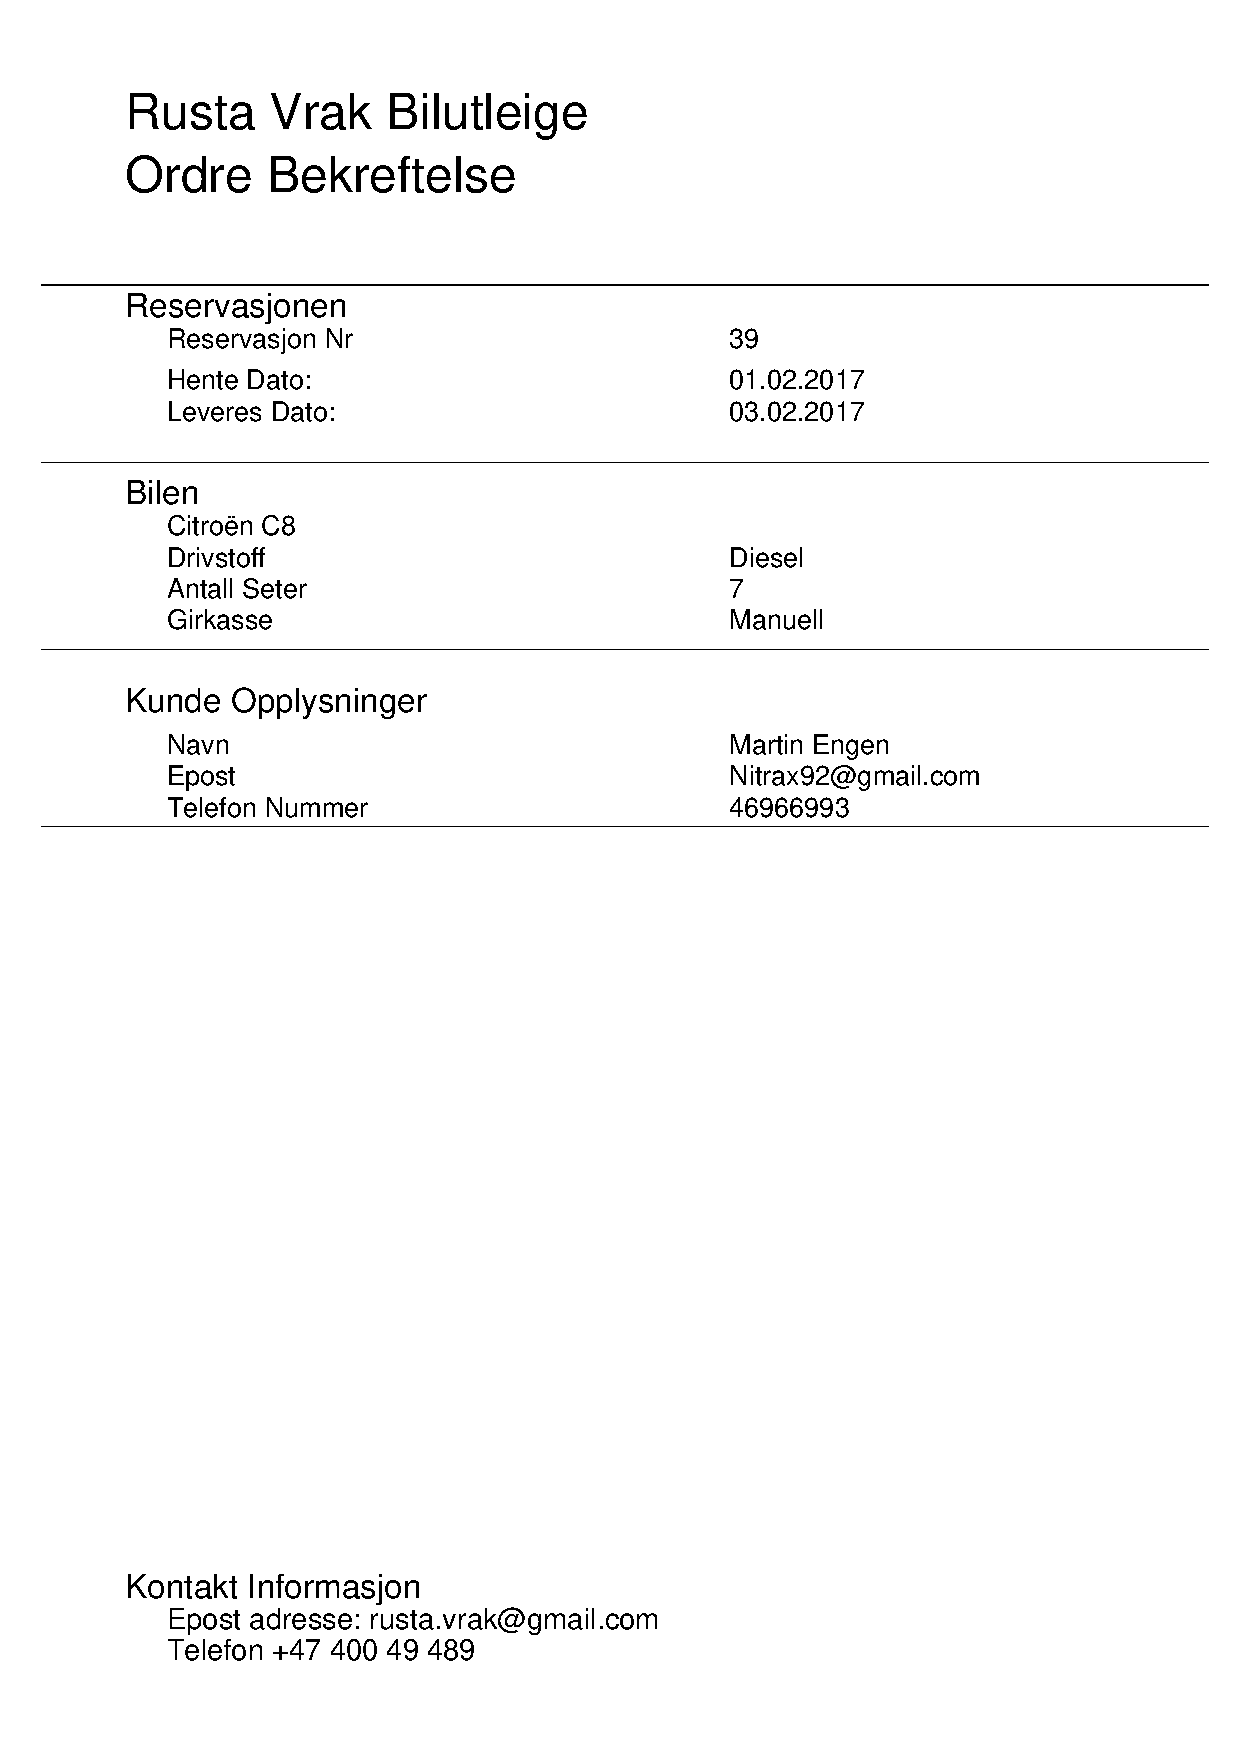
\includepdf[pages=-,landscape=false,offset=75 -75, scale=0.8, pagecommand={\thispagestyle{fancy}}]{./Appendices/rv_bekreftelse.pdf}

\lhead{Vedlegg C - Database}
\includepdf[pages=-,landscape=false,offset=75 -75, pagecommand={\thispagestyle{fancy}}]{./Appendices/database.pdf}

\addtocontents{toc}{\vspace{2em}} % Add a gap in the Contents, for aesthetics

\backmatter



\end{document}  